\documentclass[a4paper]{article} %format de la feuille + type de document https://en.wikibooks.org/wiki/LaTeX/Document_Structure#Document_classes
%packages nécessaire pour nos besoins
\usepackage[utf8]{inputenc}
\usepackage[T1]{fontenc}
\usepackage[english,french]{babel}
\usepackage{amsmath}
\usepackage{amssymb,amsfonts,textcomp}
\usepackage{color}
\usepackage[dvipsnames]{xcolor}
\usepackage{array}
\usepackage{supertabular}
\usepackage{hhline}
\usepackage{hyperref}
\usepackage{capt-of}
\usepackage[pdftex]{graphicx}
\usepackage{sectsty}
\usepackage[most]{tcolorbox}
\usepackage{textcomp}
\usepackage{courier}
\usepackage[font={small,it}]{caption}
\usepackage{float}
\usepackage{graphicx}
\usepackage{subcaption}
\usepackage{caption}


%Définition des couleurs
\definecolor{havelockBlue}{rgb}{0.004, 0.42, 0.73}
\definecolor{Monokaimagenta}{rgb}{0.86,0.08,0.24}

%utilisation de la couleur définie avant
%toutes les sections auront cette couleur
\sectionfont{\color{havelockBlue}}
\subsectionfont{\color{havelockBlue}}

\newcommand{\red}[1]{\textbf{\textcolor{OrangeRed}{#1}}}

%début du document
\begin{document}

%début d'un titre
\begin{titlepage}
            %centre les éléments
	\centering
	
	{\scshape\LARGE \color{Monokaimagenta} Laboratoire \\ Universal Asynchronous Receiver Transmitter \par}
	
	%espace vertical de 1 mms
	\vspace{1cm}
	
	{\Large\itshape Yohann Meyer \& Joel Schär\par}
	
	%http://www.personal.ceu.hu/tex/spacebox.htm
	\vfill
	Professeur\par
	%met le texte en gras 
	\textbf{Carlos Andrés Pena} \par% ajoute une ligne 
	\vspace{1cm}
	Assistant\par
	\textbf{Gaëtan Matthey}
	
	\vfill

            %affiche la date actuelle
	{\large \today\par}
	
%fin de la page de titre
\end{titlepage}

%démarre un chapitre, les nombres se mettent automatiquement et seront incrémenté quand un autre \section est rencontré
%voir https://en.wikibooks.org/wiki/LaTeX/Document_Structure#Sectioning_commands
\section{Description générale}
On appelle « trame » une suite de bits envoyés en série. Cette trame comprend dans l’ordre :
\begin{itemize}
\item Le « start-bit » toujours égal à 0.
\item Les bits de donnée (sur n bits) à transmettre.
\item Le bit de parité facultatif (non demandé dans ce labo).
\item Le bit de stop égal à 1.
\end{itemize}
De plus, l’état de repos de la ligne est fixé à 1.
\\ 
\begin{figure}[H]
    \centering
    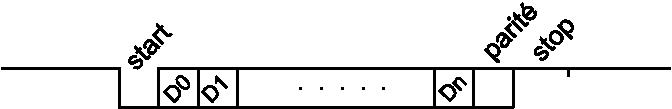
\includegraphics[width=.8\textwidth]{src/uart_1.jpg}
    \captionof{figure}{trame}
    \label{fig:trame}
\end{figure}


%saut à la ligne


%début d'un encadré avec la couleur définie plus haut
\begin{tcolorbox}[colframe=Monokaimagenta,colback=white]
\paragraph %démarre un paragraphe
{Spécification - Max 1/2 page } 
Indiquez si vous réalisez la partie émetteur ou la partie récepteur de l’UART
Placez ici les spécifications de votre circuit en décrivant son fonctionnement. Votre circuit devra être conforme à ces spécifications.\\

Nous avons réalisé la partie émetteur de l'UART. Notre circuit procède à l'envoie de 8 bits successifs donnés en entrée selon la forme demandée. Le circuit envoie la valeurs zéro sur deux temps d'horloge pour indiqué le début de l'envoi au circuit récepteur. L'envoie de chaque bits ce fait ensuite sur une durée de 4 temps d'horloge. Sur le quatrième temps l'instruction "Shift-right" est transmise au shift-register de manière a envoyer le bits suivant durant la séquence d'envoie suivante.
%fin de l'encadré
\end{tcolorbox}

\section{Architecture}\

\begin{tcolorbox}[colframe=Monokaimagenta,colback=white]
\paragraph{Architecture - Max 1/2 page}
Dessinez le schéma bloc complet de votre circuit. Ce circuit contient entre autre : shift-register, compteurs et machine d’état, avec les bus de données et les signaux de contrôle. Vous pouvez faire ce schéma bloc à la main (très proprement), ou en utilisant Logisim (mais avec le nom des signaux), ou avec un outil de dessin de votre choix.

Remplacez le texte ci-dessus par vos réponses (à l’intérieur du cadre rouge)\\

\red{Schéma final de l'UART : A REMPLACER}\\

\begin{figure}[H]
	\centering
	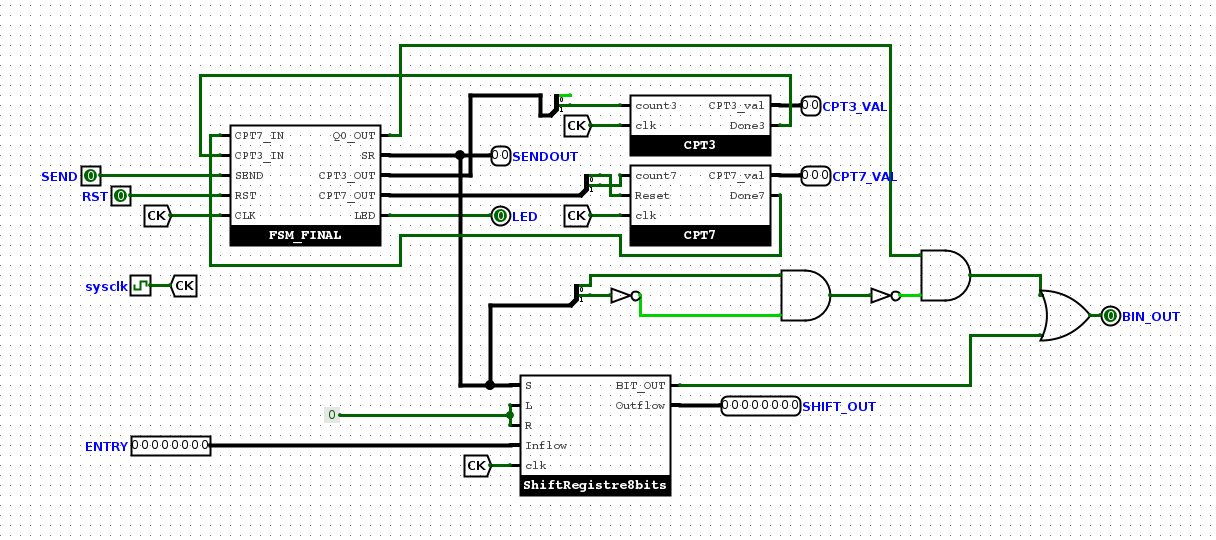
\includegraphics[width=\textwidth]{src/schema_UART}
	\captionof{figure}{UART}
	\label{fig:UART}
\end{figure}


\end{tcolorbox}


\section {Réalisation}
\subsection{Le bloc shift-register}
Ce bloc sur 8 bits a 4 modes de fonctionnement. Vous devez le refaire entièrement avec des bascules et des multiplexeurs.

\begin{tcolorbox}[colframe=Monokaimagenta,colback=white, breakable, enhanced]
\paragraph{Conception et tests - Max 1 page}
Insérez une capture d’écran pour présenter votre bloc shift-register. Expliquez brièvement son fonctionnement.
Indiquez comment vous avez testé les 4 modes de fonctionnement afin de le valider.
Remplacez le texte ci-dessus par vos réponses (à l’intérieur du cadre rouge)\\

\begin{figure}[H]
	\centering
	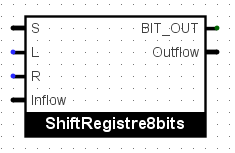
\includegraphics[scale=0.5]{src/SR_8b_bloc}
	\captionof{figure}{Bloc du Shift Register 8 bits}
	\label{fig:SR_8b_bloc}
\end{figure}
Nous avons pour le bloc Shift Register 8 bits les entrées, sorties suivantes : 
\begin{itemize}
	\item Le signal de commande "S" qui donne les instructions sur le mode de fonctionnement du registre.
	\item Les entrées "L" et "R" qui permette d'entrer une valeur depuis la gauche ou la droite au moment du shift.
	\item Un bus "Inflow" qui permet d'entrer la séquence a charger.
	\item Un bus "Outflow" qui prend les valeurs des huit état du registre.
	\item Le bit de sortie qui prend la valeur du bit de poids faible en sortie du registre.
\end{itemize}

Le signal de commande est codés comme suit :
\begin{center}
	\begin{tabular}{c|l}
		00	&	Hold\\
		01	&	Load\\
		10	&	Shift Right\\
		11	&	Shift Left\\
	\end{tabular}
\end{center}

Le shift register 8 bits que nous avons conçu est une combinaison de deux shift Register 4 bits interconnectés. 
\begin{figure}[H]
	\centering
	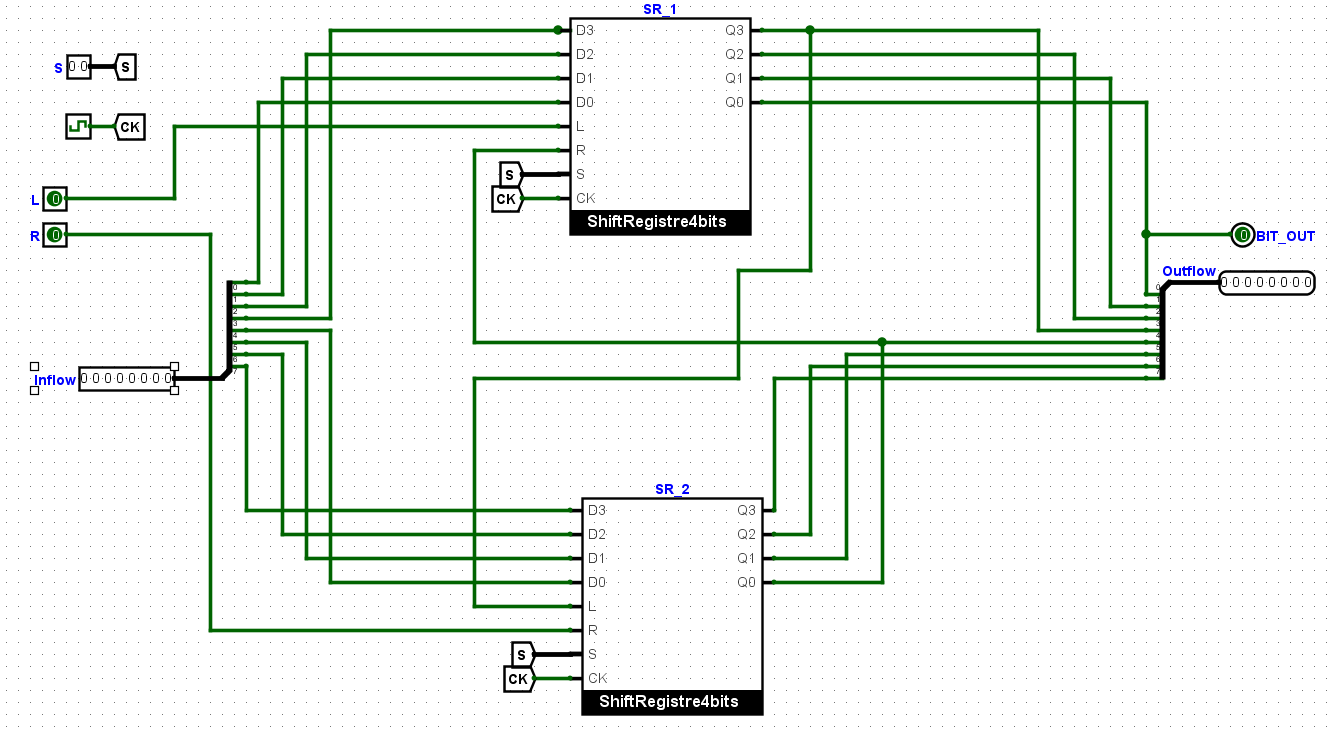
\includegraphics[width=\textwidth]{src/SR_8b}
	\captionof{figure}{Shift Register 8 bits}
	\label{fig:SR_8b}
\end{figure}
Le registre "SR\_2" a 4bits prend en entrée les bits de poids fort (gauche) du flux d'entrée. Il transmet sont bit de poids faible Q0 au second registre "SR\_1" qui traite les bits de poids faible. La flux "ouflow" de sortie est la combinaison des sortie "Q0-Q3" des deux blocs et le "bit-out" le bit de poids faible de cette séquence.

Chaque "shift register" à 4bits et structuré comme suit.
\begin{figure}[H]
	\centering
	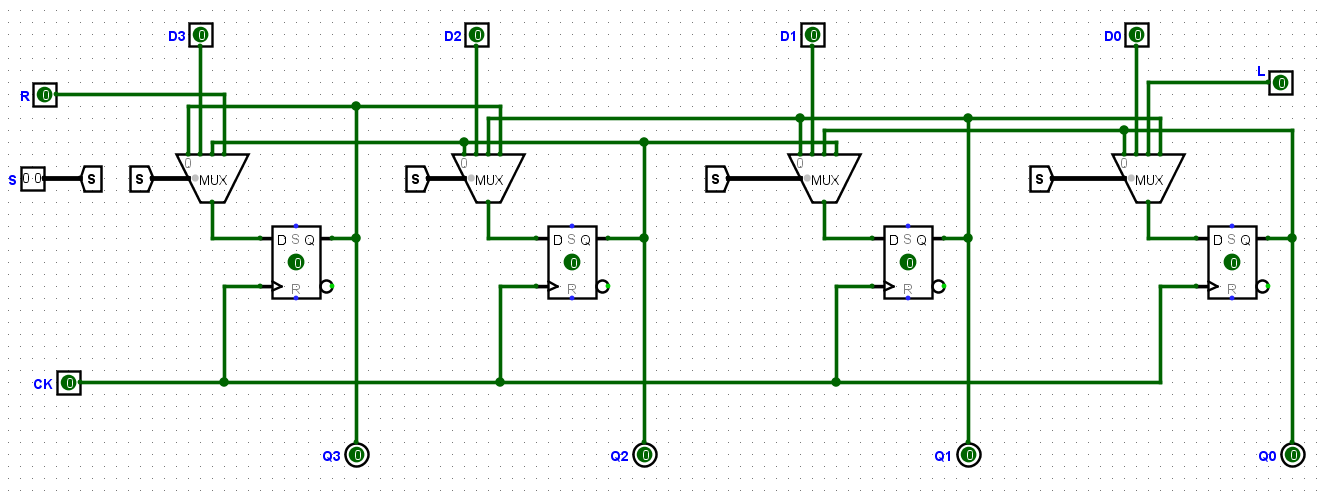
\includegraphics[width=\textwidth]{src/SR_4b}
	\captionof{figure}{Shift Register 4 bits}
	\label{fig:SR_4b}
\end{figure}
Chaque bascule prend en entrée la valeur donnée par un multiplexer en fonction du code de commande. Cette valeur est la valeur du bit donné par le flux d'entrée ("inflow" : Shift Register 8bits) au moment de la commande "Load" (01). La valeur de l'état "Q+1" lors d'un "Shift Left" (10). La valeur de l'état "Q-1" lors d'un "Shift Right" (11). La valeur "Q" actuelle en mode "Hold" (00). Le changement se fait à chaque flanc montant de l'horloge.
\end{tcolorbox}

\subsection{Le bloc compteur 0-3}
Le premier compteur demandé compte de 0 à 3. Ce compteur comprend une entrée de remise à 0 synchrone et une sortie indiquant que le compteur a atteint sa valeur maximum.

\begin{tcolorbox}[colframe=Monokaimagenta,colback=white, breakable, enhanced]
\paragraph{Conception et tests - Max 1 page }
Insérez une capture d’écran pour présenter votre bloc compteur 0-3. Expliquez sa réalisation et son fonctionnement.
Indiquez comment vous avez testé les différents modes de fonctionnement afin de le valider. Vous pouvez ajouter un chronogramme.
Remplacez le texte ci-dessus par vos réponses (à l’intérieur du cadre rouge)\\

\red{Notre compteur n'a pas l'entrée de remise à zéro synchrone. Il se remet à zéro d'office quand on ne compte pas.}\\

Le compteur 0-3 que nous avons implémenté, reçoit comme entrées l'indication de compter, et transmet en sortie la valeur à laquelle il se trouve ainsi qu'un bit indiquant le compteur à terminé de compter jusqu'à 3.\\	
\begin{figure}[H]
	\centering
	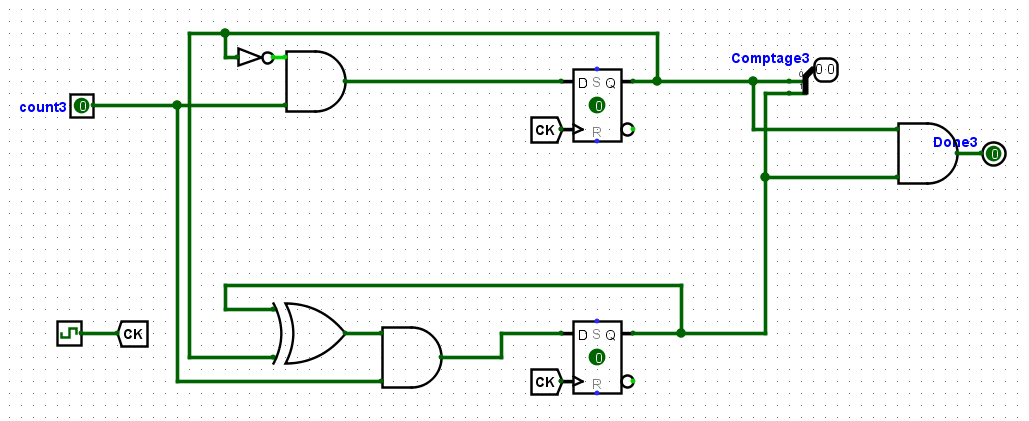
\includegraphics[width=\textwidth]{src/CPT_03_1}
	\captionof{figure}{Compteur de 0 à 3}
	\label{fig:CPT_03_1}
\end{figure}
Selon les besoins du laboratoire et pour des raison d'optimisation si la valeur d'entrée n'est pas à 1 et ne donne pas l'ordre de compter, le compteur se remet automatiquement à 0. Il est donc prêt à recommencer une séquence. Nous n'avons jamais besoin d'interrompre ce compteur et de garder sa valeur en mémoire. L'utilisation d'une commande de remise à zéro est donc superflue.\\

\begin{figure}[H]
	\centering
	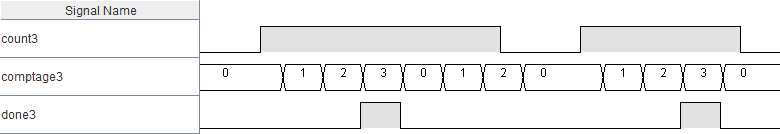
\includegraphics[width=\textwidth]{src/chrono_CPT3_1}
	\captionof{figure}{Chronogram Compteur de 0 à 3}
	\label{fig:chrono_CPT_03_1}
\end{figure}
Ce chronogram illustre le fonctionnement du compteur et met en évidence la remise à zéro automatique du compteur.

\red{Si tu as encore ton schéma ou ta table d'état sur la base du quel t'as conçu le compteur il faudrait le mettre sinon on le refera.}\\

Pour des raisons de conception de notre machine d'état, la transition entre l'état dans lequel le compteur compte et le celui ou le shift de la valeur se fait, nécessite un battement d'horloge. De ce fait nous avons utilisé un compteur qui donne l'indication de fin de comptage a 2 et non 3.
\begin{figure}[H]
	\centering
	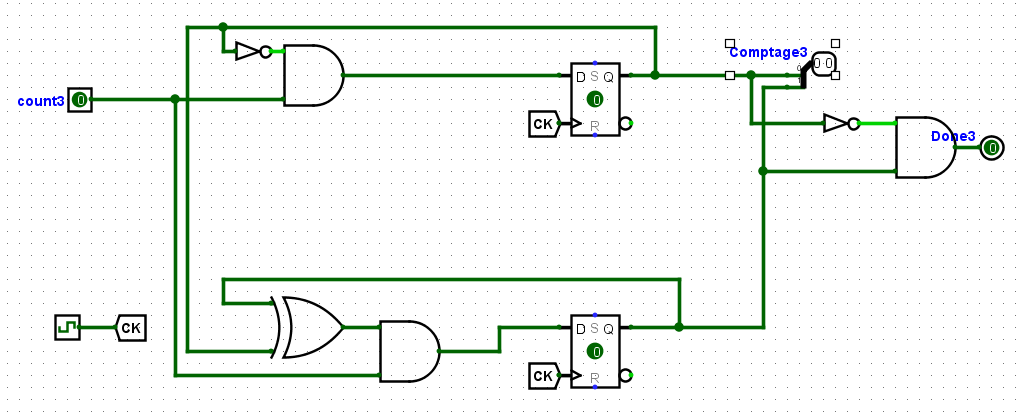
\includegraphics[width=\textwidth]{src/CPT_03_2}
	\captionof{figure}{Compteur de 0 à 2}
	\label{fig:CPT_03_2}
\end{figure}
\end{tcolorbox}

\subsection{Le bloc compteur 0-7}
Le deuxième compteur demandé compte de 0 à 7. Ce compteur comprend une entrée de remise à 0 synchrone, une entrée enable pour l’activer et une sortie indiquant que le compteur a atteint sa valeur maximum.

\begin{tcolorbox}[colframe=Monokaimagenta,colback=white, breakable, enhanced]
\paragraph{Conception et tests - Max 1 page}
Insérez une capture d’écran pour présenter votre bloc compteur 0-7. Expliquez sa réalisation et son fonctionnement. Inutile de reprendre les explications du paragraphe précédent 3.2. Expliquez simplement ce que vous avez dû changer ou rajouter pour passer du compteur 0-3 au compteur 0-7.
Indiquez comment vous avez testé les différents modes de fonctionnement afin de le valider. Vous pouvez ajouter un chronogramme.
Remplacez le texte ci-dessus par vos réponses (à l’intérieur du cadre rouge)\\

Le compteur 7 que nous avons implémenté nous permet de compter le nombre de bits qui on été envoyé, de manière à savoir quand la séquence de 8 bits à été envoyée au complet.\\
Ce compteur doit donc garder la valeur en mémoire quand l'ordre le bit "count" est a zéro et reprendre dans le cas contraire. Il est donc également nécessaire d'avoir une entrée "reset" qui permet de le remettre à 0.\\
\begin{figure}[H]
	\centering
	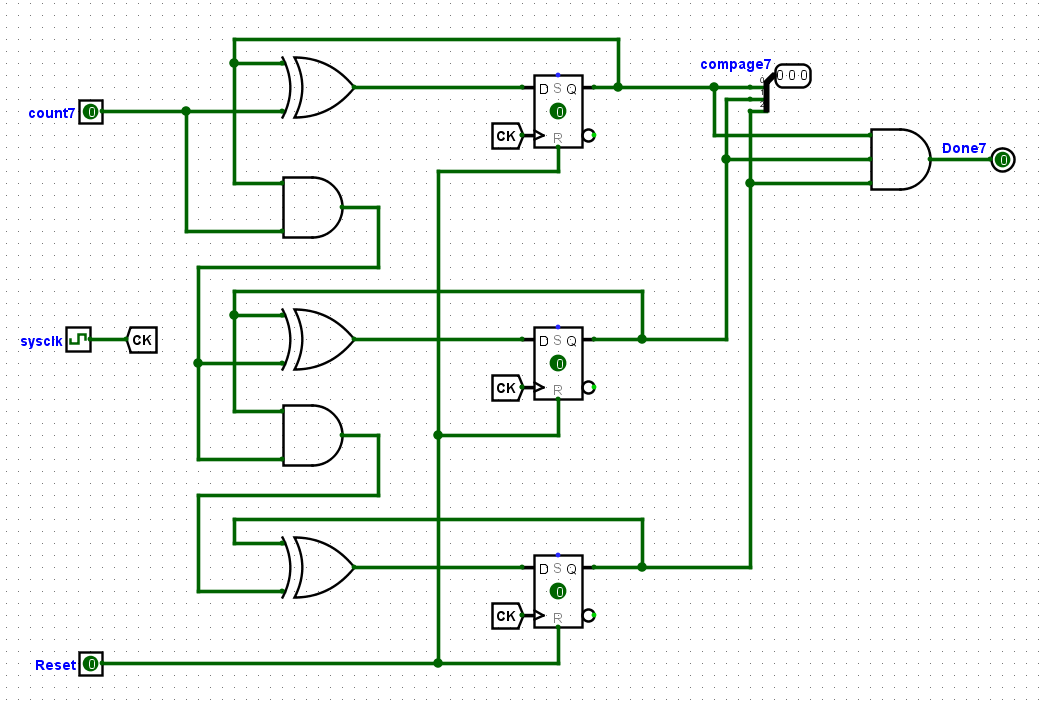
\includegraphics[width=\textwidth]{src/CPT_07}
	\captionof{figure}{Compteur de 0 à 7}
	\label{fig:CPT_07}
\end{figure}
	


\end{tcolorbox}

\subsection{La machine d’état}
Cette machine d’état de type 1 parmi M contrôle les deux compteurs et le shift register. 
\begin{tcolorbox}[colframe=Monokaimagenta,colback=white, breakable, enhanced]
\paragraph{Conception Max 3 pages}
Précisez les entrées et sorties de votre machine d’état
Insérez un graphe des états et une table des états. Donnez des explications sur le fonctionnement de votre machine. Quel est son Type ?
Donnez les équations des états futurs et insérez une capture d’écran de la réalisation de votre machine.
Remplacez le texte ci-dessus par vos réponses (à l’intérieur du cadre rouge)
\\
\end{tcolorbox}
\section {Intégration et simulation}
\subsection{Intégration}
Suivant votre partie à concevoir, vous devez réalisé l’UART en interconnectant les différents blocs. 
\begin{tcolorbox}[colframe=Monokaimagenta,colback=white, breakable, enhanced]
\paragraph{Réalisation et simulation Logisim - Max 1 page}
Insérez une capture d’écran de l’UART complet sous Logisim
Expliquez le fonctionnement global de l’UART
Remplacez le texte ci-dessus par vos réponses (à l’intérieur du cadre rouge)
\\
\end{tcolorbox}
 \subsection{Simulation sous Logisim}
L’UART réalisé est ensuite testé en simulation sous Logisim.
\begin{tcolorbox}[colframe=Monokaimagenta,colback=white, breakable, enhanced]
\paragraph{Réalisation et simulation Logisim - Max 2 pages}
Indiquez comment vous simulez votre UART sous Logisim (seul ou avec le générateur fourni), ET avec un UART d’un autre groupe (indiquez quel groupe)
Insérez un ou plusieurs chronogrammes, annotez-le(s) et expliquez pourquoi le fonctionnement est correct et conforme aux spécifications.
Remplacez le texte ci-dessus par vos réponses (à l’intérieur du cadre rouge)
\\
\end{tcolorbox}
 \subsection{Synthèse et test de fonctionnement réel}
Synthèse et configuration du matériel, test de fonctionnement.
L’UART finalement synthétisé et chargé dans une carte, une carte émetteur sera reliée à une carte récepteur afin de tester une transmission de données.
\begin{tcolorbox}[colframe=Monokaimagenta,colback=white, breakable, enhanced]
\paragraph{Essais avec une carte - Max 1 page}
Indiquez comment vous faites le test (et avec un groupe différent de la simulation). Quelles données choisissez-vous pour faire les essais ?Vous devez faire valider votre circuit en fonctionnement au professeur ou à l’assistant
Commentez brièvement votre expérience dans cette étape en mentionnant, par exemple, des éventuelles difficultés à faire fonctionner le circuit ou à configurer la carte, etc.
Remplacez le texte ci-dessus par vos réponses (à l’intérieur du cadre rouge)
\\
\end{tcolorbox}
\section {Conclusion}
\begin{tcolorbox}[colframe=Monokaimagenta,colback=white, breakable, enhanced]
\paragraph{Conclusion - Max 1/2 page}
Cette section est libre pour que vous fassiez une analyse critique de votre laboratoire
Commentez et analysez 
les résultats, 
les difficultés et les succès
Rédigez quelques conclusions personnelles
Donnez vos impressions et analysez votre expérience dans ce laboratoire
Discutez de ce que vous avez appris (ou pas)
Analysez votre travail, votre implication
Evitez les banalités et les lieux communs
ETCAETERA…
\\
\end{tcolorbox}

\end{document}